% Provenance (never printed): see sources/outline_sources.md (Year 1: insolation with
% latitude and season, the radiative surplus and deficit, meridional heat transport by
% the atmosphere and the ocean, latent heat). Exercise and problem values in the Book 3
% scratch calculator calc/ch27.py; figures from figdata/bachelor-1/insolation.py (Kepler
% orbit of _solar.py) and energy_balance.py (NCEP-NCAR Reanalysis 1, long-term means
% 1991-2020, datasets bachelor-1-ncep-*).
% Physics owns the inverse-square law, the black body and the Stefan-Boltzmann law, the
% seasons and latent heat (recalled). Book 2 (g10) gave the quarter of the solar constant,
% the global budget diagram and its closure, latent and sensible heat in words, the
% annual-mean insolation curve and the poleward transport in words: re-founded here with
% derivations and data. Ch. 1 gave the instantaneous insolation, the declination and the
% rising and setting of the Sun.
\chapter{विकिरण और ऊष्मा का परिवहन}\label{ch:b1:radiation-heat-transport}

एक लाख मील दूर से पृथ्वी का धूप वाला चेहरा नीले समुद्र, भूरी भूमि और सफ़ेद बादलों की एक डिस्क है। सूर्य का प्रकाश डिस्क के मध्य पर, उष्णकटिबंध के निकट, सबसे सीधा पड़ता है और उसके किनारों को छूकर निकलता है; उष्णकटिबंध ध्रुवीय क्षेत्रों से कहीं अधिक ऊर्जा सोखते हैं। फिर भी उष्णकटिबंध साल-दर-साल गरम नहीं होते, न ध्रुव ठंडे। पवनें और महासागरीय धाराएँ अतिरिक्त ऊर्जा को ध्रुवों की ओर ले जाती हैं, कई पेटावाट। यह अध्याय उस संतुलन के तीन पदों को मापता है: हर \omterm{def:b1:spherical-astronomy:geographic}{अक्षांश} को मिलने वाला सूर्य का प्रकाश, वह भाग जो वह रखता है और वह अवरक्त जो वह अंतरिक्ष को लौटाता है, और वह परिवहन जो अंतर को पूरा करता है। परिवहन का एक बड़ा भाग एक अदृश्य रूप में चलता है, जल-वाष्प के रूप में, जिसकी गुप्त ऊष्मा वहाँ छूटती है जहाँ वह वर्षा में संघनित होती है।
% ledger: commons:epic-earth, trenberth:transport

\begin{omfigure}
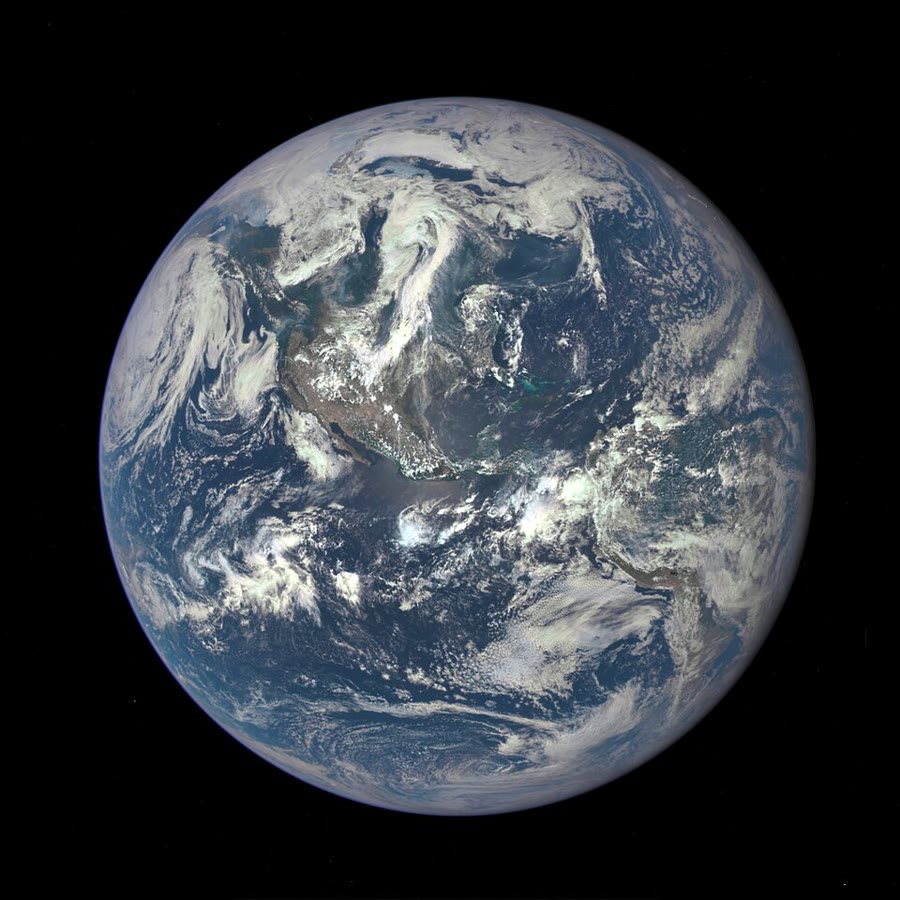
\includegraphics[width=0.55\linewidth]{images/book3/b1-epic-earth.jpg}

{\small सूर्य-प्रकाश से प्रकाशित पृथ्वी का पूरा भाग, 6 जुलाई 2015 को डीप स्पेस क्लाइमेट ऑब्ज़र्वेटरी के एक कैमरे से एक लाख मील दूर से खींचा गया; उत्तर और मध्य अमेरिका बीच में हैं, कैरिबियन के फ़िरोज़ी उथले सागरों के साथ। जून संक्रांति के दो सप्ताह बाद ऊपर का आर्कटिक चौबीसों घंटे प्रकाशित है। चमकीले बादल उन तक पहुँचने वाले प्रकाश का बड़ा भाग परावर्तित करते हैं; नीला आभास वायु के अणुओं द्वारा बिखेरा गया सूर्य का प्रकाश है। (फ़ोटो: NASA Goddard Space Flight Center, सार्वजनिक डोमेन, विकिमीडिया कॉमन्स के माध्यम से।)}
\label{fig:b1:radiation-heat-transport:epic}
\end{omfigure}
% ledger: commons:epic-earth (polar day: figdata/bachelor-1/insolation.py)

\begin{recall}
\Cref{ch:b1:spherical-astronomy} ने प्रति वर्ग मीटर उस सूर्य-प्रकाश की शक्ति के रूप में अंतर्ग्रहण को परिभाषित किया, जो वायुमंडल के ऊपरी भाग में एक क्षैतिज सतह के प्रति वर्ग मीटर पर पड़ती है, $I = S_0(a/r)^2\sin h_\odot$ जब सूर्य ऊपर है, $S_0 = \qty{1361}{W.m^{-2}}$ के साथ माध्य दूरी $a$ पर; उसने सूर्य की ऊँचाई उसके घंटा-कोण $H$, उसके क्रांति-कोण $\delta$ और \omterm{def:b1:spherical-astronomy:geographic}{अक्षांश} $\varphi$ से दी,
$\sin h_\odot = \sin\varphi\sin\delta + \cos\varphi\cos\delta\cos H$; और सूर्यास्त का घंटा-कोण $H_0$, $\cos H_0 = -\tan\varphi\tan\delta$ (\cref{prop:b1:spherical-astronomy:rising})। \Cref{ch:b1:comparative-planetology} ने ग्रह का \omterm{def:b1:comparative-planetology:albedo}{बॉन्ड एल्बिडो} और उसका संतुलन तापमान परिभाषित किया। भौतिकी खंड प्रकाश के लिए व्युत्क्रम-वर्ग नियम देते हैं, कृष्णिका का विकिरण, प्रति वर्ग मीटर $\sigma T^4$ जिसमें $\sigma = \qty{5.670e-8}{W.m^{-2}.K^{-4}}$ है (स्टीफ़न–बोल्ट्ज़मान), और अवस्था-परिवर्तन की गुप्त ऊष्मा। पुस्तक~2 ने दिखाया कि पृथ्वी औसतन सौर स्थिरांक का एक-चौथाई ग्रहण करती है, पृथ्वी का वैश्विक ऊर्जा-बजट बनाया और जाँचा कि वह संतुलित है, और ऊष्मा के ध्रुवोन्मुखी परिवहन का शब्दों में वर्णन किया।
% ledger: earth:TSI, const:sigma, ipcc:budget-toa
\end{recall}

\section{अक्षांश और मौसम के साथ अंतर्ग्रहण}\label{sec:b1:radiation-heat-transport:insolation}

तात्कालिक अंतर्ग्रहण हर मिनट बदलता है क्योंकि सूर्य आकाश पार करता है। जलवायु के लिए जो मायने रखता है वह एक दिन पर उसका योग है।

\begin{definition}[दैनिक-माध्य अंतर्ग्रहण]\label{def:b1:radiation-heat-transport:daily-insolation}
एक दिन पर किसी \omterm{def:b1:spherical-astronomy:geographic}{अक्षांश} का \emph{दैनिक-माध्य अंतर्ग्रहण}\index{दैनिक-माध्य अंतर्ग्रहण} $\bar Q$ उस दिन के 24 घंटों पर औसत किया गया तात्कालिक अंतर्ग्रहण है, रातों समेत, सूर्य का क्रांति-कोण और उसकी दूरी उस दिन के मानों पर रखे हुए। यह वायुमंडल के ऊपरी भाग में क्षैतिज सतह के प्रति वर्ग मीटर की शक्ति है, \unit{W.m^{-2}} में।
\end{definition}

एक दिन के लिए $\delta$ और $r$ को स्थिर रखना हानिरहित है: क्रांति-कोण एक दिन में अधिकतम \ang{0.4} बदलता है, और दूरी \qty{0.03}{\percent} से कम।
% ledger: earth:obliquity, earth:ecc (computed in figdata/bachelor-1/insolation.py)

\begin{theorem}[दैनिक-माध्य अंतर्ग्रहण]\label{thm:b1:radiation-heat-transport:daily}
\omterm{def:b1:spherical-astronomy:geographic}{अक्षांश} $\varphi$ पर, एक ऐसे दिन पर जब सूर्य का क्रांति-कोण $\delta$ और उसकी दूरी $r$ है,
\[
  \bar Q = \frac{S_0}{\pi}\left(\frac{a}{r}\right)^{2}
  \bigl(h_0\sin\varphi\sin\delta + \cos\varphi\cos\delta\sin h_0\bigr),
\]
जहाँ $h_0 \in [0, \pi]$ रेडियन में सूर्यास्त का घंटा-कोण है: $\cos h_0 =
-\tan\varphi\tan\delta$ जब $|\tan\varphi\tan\delta| \le 1$; $h_0 = \pi$ ध्रुवीय दिवस में ($\tan\varphi\tan\delta > 1$); $h_0 = 0$, और $\bar Q = 0$, ध्रुवीय रात में ($\tan\varphi\tan\delta < -1$)।
\end{theorem}

\begin{proof}
घंटा-कोण $H$ एक दिन में समान रूप से $2\pi$ तक आगे बढ़ता है, इसलिए दिन पर माध्य $H \in [-\pi, \pi]$ पर माध्य है। सूर्य $-h_0 < H < h_0$ के लिए ऊपर है, जहाँ $\sin h_\odot > 0$ है, और अन्यथा अंतर्ग्रहण शून्य है। अतः
\[
  \bar Q = \frac{1}{2\pi}\int_{-h_0}^{h_0} S_0\left(\frac{a}{r}\right)^{2}
  \bigl(\sin\varphi\sin\delta + \cos\varphi\cos\delta\cos H\bigr)\,\mathrm dH ,
\]
जो $(S_0/2\pi)(a/r)^2\bigl(2h_0\sin\varphi\sin\delta +
2\cos\varphi\cos\delta\sin h_0\bigr)$ है।
सीमाएँ \cref{prop:b1:spherical-astronomy:rising} से आती हैं: ऊँचाई शून्य है जब $\cos H = -\tan\varphi\tan\delta$। यदि वह संख्या निरपेक्ष मान में 1 से अधिक है, तो सूर्य कभी क्षितिज पार नहीं करता: जब $\tan\varphi\tan\delta > 1$, समाकलन-फलन हर $H$ के लिए धनात्मक है और समाकलन पूरे दिन पर चलता है, $h_0 = \pi$; जब $\tan\varphi\tan\delta < -1$, वह हर $H$ के लिए ऋणात्मक है और सूर्य कभी नहीं उगता।
\end{proof}

दो विशेष स्थितियाँ याद रखने योग्य हैं। भूमध्य रेखा पर, $\varphi = 0$ और $h_0 = \pi/2$, मौसम चाहे जो हो:
\[
  \bar Q_\text{भूमध्य रेखा} = \frac{S_0}{\pi}\left(\frac{a}{r}\right)^{2}\cos\delta ,
\]
माध्य दूरी पर $S_0/\pi = \qty{433.2}{W.m^{-2}}$ के साथ, सम-रात्रियों पर सबसे बड़ी। ध्रुव पर उसकी गर्मी में, $h_0 = \pi$ और $\varphi = \pi/2$: $\bar Q_\text{ध्रुव} =
S_0(a/r)^2\sin\delta$, सूर्य आकाश में एक स्थिर ऊँचाई पर घूमता है जो क्रांति-कोण के बराबर है।
% ledger: earth:TSI

\begin{proposition}[ध्रुवीय ग्रीष्म]\label{prop:b1:radiation-heat-transport:polar-summer}
क्रांति-कोण $\delta > 0$ के एक दिन पर, उत्तरी ध्रुव पर \omterm{def:b1:radiation-heat-transport:daily-insolation}{दैनिक-माध्य अंतर्ग्रहण} भूमध्य रेखा के अंतर्ग्रहण से तभी अधिक है यदि और केवल यदि $\pi\tan\delta > 1$ है, अर्थात् $\delta >
\ang{17.66}$। जून संक्रांति पर, $\delta = \ang{23.44}$, अनुपात $\pi\tan
\delta = 1.362$ है।
\end{proposition}

\begin{proof}
ऊपर की दो विशेष स्थितियाँ गुणक $(S_0/\pi)(a/r)^2$ साझा करती हैं; उनका अनुपात $\pi\sin\delta/\cos\delta = \pi\tan\delta$ है, जो 1 से अधिक है जब $\tan\delta >
1/\pi$, $\delta > \arctan(1/\pi) = \ang{17.66}$। तिरछेपन के साथ, $\pi\tan\ang{23.44} = 1.362$।
\end{proof}
% ledger: earth:obliquity

पृथ्वी की कक्षा के साथ, जून संक्रांति अपसौर के निकट पड़ती है, $(a/r)^2 = 0.968$: उत्तरी ध्रुव तब दैनिक माध्य के रूप में \qty{524}{W.m^{-2}} पाता है, भूमध्य रेखा \qty{385}{W.m^{-2}}। छह महीने बाद दक्षिणी ध्रुव, उपसौर के निकट, \qty{559}{W.m^{-2}} पाता है, उत्तरी ध्रुव को उसकी गर्मी में मिली राशि से \qty{6.7}{\percent} अधिक: अनुपात ठीक $(a/r)^2$ के दो मानों का अनुपात है। नीचे का चित्र पूरे वर्ष भर में $\bar Q$ दिखाता है। शिखर संक्रांतियों पर ध्रुवों पर हैं; गहरी फाँकें ध्रुवीय रातें हैं, \omterm{def:b1:spherical-astronomy:geographic}{अक्षांश} $\ang{90} -
|\delta|$ से सीमित; उपसौर बिंदु, जहाँ दोपहर को सूर्य सिर के ऊपर से गुज़रता है, क्रांति-कोण के साथ उष्णकटिबंधों के बीच चलता है।
% ledger: earth:TSI, earth:ecc, earth:obliquity, nasa:earth-perihelion-longitude, usno:seasons-2026 (computed in figdata/bachelor-1/insolation.py)

\begin{omfigure}
\begin{tikzpicture}
\begin{axis}[omrecord, width=0.8\linewidth, height=6.4cm, view={0}{90},
  xmin=0, xmax=365, ymin=-90, ymax=90, xlabel={वर्ष का दिन (1 जनवरी से)},
  ylabel={अक्षांश (\unit{\degree})}, xtick={0,60,...,360}, ytick={-90,-60,...,90},
  colormap/viridis, colorbar, point meta min=0, point meta max=560,
  colorbar style={ylabel={$\bar Q$ (\unit{W.m^{-2}})}, ytick={0,100,...,500}, width=0.3cm},
  axis on top, grid=none]
% figdata/bachelor-1/insolation.py; ledger: earth:TSI, earth:ecc, earth:obliquity, nasa:earth-perihelion-longitude, usno:tropical-year, usno:seasons-2026
\addplot3[surf, shader=interp, mesh/ordering=y varies, mesh/rows=73]
  table[x=day, y=lat, z=Q] {figdata/out/bachelor-1-insolation-grid.dat};
\addplot3[white, dashed, line width=0.8pt] table[x=day, y=decl, z expr=600] {figdata/out/bachelor-1-insolation-sun.dat};
\addplot3[white, line width=0.6pt, unbounded coords=jump] table[x=day, y=night_n, z expr=600] {figdata/out/bachelor-1-insolation-sun.dat};
\addplot3[white, line width=0.6pt, unbounded coords=jump] table[x=day, y=night_s, z expr=600] {figdata/out/bachelor-1-insolation-sun.dat};
\node[font=\scriptsize, text=white] at (axis cs:28,81,700) {ध्रुवीय रात};
\node[font=\scriptsize, text=white] at (axis cs:172,-81,700) {ध्रुवीय रात};
\node[font=\scriptsize, text=white, anchor=south] at (axis cs:172,26,700) {उपसौर अक्षांश};
\end{axis}
\end{tikzpicture}

{\small \omterm{def:b1:radiation-heat-transport:daily-insolation}{दैनिक-माध्य अंतर्ग्रहण}, वायुमंडल के ऊपरी भाग पर, वर्ष के दिन और \omterm{def:b1:spherical-astronomy:geographic}{अक्षांश} के विरुद्ध, \cref{thm:b1:radiation-heat-transport:daily} से $S_0 = \qty{1361}{W.m^{-2}}$ और पृथ्वी की कक्षा के साथ। धराशायी: उपसौर \omterm{def:b1:spherical-astronomy:geographic}{अक्षांश}, जो क्रांति-कोण के बराबर है; ठोस: ध्रुवीय रातों के किनारे। ग्रीष्म के ध्रुव पृथ्वी पर किसी भी अन्य स्थान से अधिक पाते हैं; दक्षिणी गर्मी, उपसौर के निकट, दोनों में चमकीली है।}
\label{fig:b1:radiation-heat-transport:matrix}
\end{omfigure}
% ledger: earth:TSI, earth:ecc, earth:obliquity, nasa:earth-perihelion-longitude, usno:seasons-2026

वर्ष-भर $\bar Q$ का माध्य लेकर हर \omterm{def:b1:spherical-astronomy:geographic}{अक्षांश} का वार्षिक-माध्य अंतर्ग्रहण मिलता है (नीचे का चित्र): भूमध्य रेखा पर \qty{415.6}{W.m^{-2}}, \ang{40} पर \qty{328.3}{W.m^{-2}}, किसी ध्रुव पर \qty{172.4}{W.m^{-2}}। ध्रुवीय ग्रीष्म तीव्र है पर ध्रुवीय शीत अंधेरी है, और वर्ष भर भूमध्य रेखा किसी ध्रुव से \num{2.41} गुना अधिक पाती है। वक्र दोनों गोलार्धों में एक ही है, यद्यपि दक्षिणी ग्रीष्म अधिक चमकीली है; \cref{exo:b1:radiation-heat-transport:10} बताता है कि क्यों।
% ledger: earth:TSI, earth:ecc, earth:obliquity (computed in figdata/bachelor-1/insolation.py)

\begin{omfigure}
\begin{tikzpicture}
\begin{axis}[omrecord, width=0.8\linewidth, height=5.6cm, xmin=-90, xmax=90, ymin=0, ymax=600,
  xlabel={अक्षांश (\unit{\degree})}, ylabel={$\bar Q$ (\unit{W.m^{-2}})},
  xtick={-90,-60,...,90}, ytick={0,100,...,600}]
% figdata/bachelor-1/insolation.py; ledger: earth:TSI, earth:ecc, earth:obliquity, nasa:earth-perihelion-longitude
\addplot[omThm, line width=0.8pt] table[x=lat, y=Q_jun] {figdata/out/bachelor-1-insolation-annual.dat};
\addplot[omDef, line width=0.8pt] table[x=lat, y=Q_dec] {figdata/out/bachelor-1-insolation-annual.dat};
\addplot[black, line width=1.1pt] table[x=lat, y=Q_ann] {figdata/out/bachelor-1-insolation-annual.dat};
\addplot[black!60, dashed, domain=-90:90] {340.30};
\node[font=\scriptsize, text=omThm, anchor=west] at (axis cs:50,540) {जून संक्रांति};
\node[font=\scriptsize, text=omDef, anchor=east] at (axis cs:-50,575) {दिसंबर संक्रांति};
\node[font=\scriptsize, anchor=north] at (axis cs:-72,160) {वार्षिक माध्य};
\node[font=\scriptsize, text=black!60, anchor=south west] at (axis cs:-88,342) {वैश्विक माध्य};
\end{axis}
\end{tikzpicture}

{\small दो संक्रांतियों पर \omterm{def:b1:spherical-astronomy:geographic}{अक्षांश} के विरुद्ध \omterm{def:b1:radiation-heat-transport:daily-insolation}{दैनिक-माध्य अंतर्ग्रहण}, और उसका वार्षिक माध्य (काला)। वार्षिक माध्य \qty{340.3}{W.m^{-2}} (धराशायी) के वैश्विक माध्य से अधिक है, \ang{37} दक्षिण और \ang{37} उ के बीच, पृथ्वी की सतह के \qty{60}{\percent} पर।}
\label{fig:b1:radiation-heat-transport:annual}
\end{omfigure}
% ledger: earth:TSI, earth:ecc, earth:obliquity (computed in figdata/bachelor-1/insolation.py)

\begin{proposition}[वैश्विक माध्य]\label{prop:b1:radiation-heat-transport:global}
हर क्षण, पूरे गोले पर औसत अंतर्ग्रहण $\tfrac14
S_0(a/r)^2$ है। वर्ष पर भी औसत लेने पर, वह $S_0/(4\sqrt{1 - e^2})$ है, जहाँ $e$ कक्षा की उत्केंद्रता है: पृथ्वी के लिए \qty{340.30}{W.m^{-2}}, $S_0/4 = \qty{340.25}{W.m^{-2}}$ के \qty{0.02}{\percent} के भीतर।
\end{proposition}

\begin{proof}
पृथ्वी, त्रिज्या $R$ की, क्षेत्रफल $\pi
R^2$ की एक डिस्क के आर-पार गुज़रने वाला सूर्य-प्रकाश ग्रहण करती है, शक्ति $S_0(a/r)^2\pi R^2$, जो दिवस-गोलार्ध पर पड़ती है; पूरी सतह $4\pi R^2$ पर फैलाने पर, वह पहला परिणाम देती है। कक्षा पर $(a/r)^2$ का काल-माध्य $1/\sqrt{1-e^2}$ है (\cref{exo:b1:radiation-heat-transport:11})।
\end{proof}
% ledger: earth:TSI, earth:ecc

\section{शोषित और उत्सर्जित विकिरण}\label{sec:b1:radiation-heat-transport:toa}

किसी \omterm{def:b1:spherical-astronomy:geographic}{अक्षांश} को मिलने वाले सूर्य-प्रकाश में से वह एक भाग सीधे वापस परिलक्षित करता है, बादलों, बर्फ़, हिम, रेगिस्तान और, कम मात्रा में, समुद्र से; बाकी को वह हवा में और सतह पर सोखता है। वह दिन-रात अवरक्त विकिरण द्वारा अंतरिक्ष में उत्सर्जन से भी ऊर्जा खोता है।

\begin{definition}[बाह्य दीर्घ-तरंग विकिरण]\label{def:b1:radiation-heat-transport:olr}
\emph{बाह्य दीर्घ-तरंग विकिरण}\index{बाह्य दीर्घ-तरंग विकिरण} (OLR) वायुमंडल के ऊपरी भाग से अंतरिक्ष की ओर निकलने वाले अवरक्त विकिरण की शक्ति है, प्रति वर्ग मीटर। \emph{उत्सर्जन तापमान}\index{उत्सर्जन तापमान} $T_e$ उस कृष्णिका का तापमान है जो वही शक्ति उत्सर्जित करती: $\sigma T_e^4 = \text{OLR}$।
\end{definition}

OLR कुछ भाग सतह से आता है, उस वायु के माध्यम से जो अवरक्त के लिए पारदर्शी है, और कुछ भाग ऊपर की हवा और बादलों के शिखरों से। \omterm{def:b1:radiation-heat-transport:olr}{उत्सर्जन तापमान}, जैसा नीचे परिभाषित है, विकिरण का गुण है, किसी विशेष स्तर के तापमान का नहीं: वह नीचे की ज़मीन से कम है, क्योंकि उत्सर्जित करने वाली परतें ठंडी हैं।
% ledger: ipcc:budget-surface, ipcc:budget-toa

\begin{definition}[शुद्ध विकिरण; विकिरण-आधिक्य और न्यूनता]\label{def:b1:radiation-heat-transport:net-radiation}
वायुमंडल के ऊपरी भाग पर \emph{शुद्ध विकिरण}\index{शुद्ध विकिरण} है
\[
  R = \underbrace{(1 - \alpha)\,\bar Q}_{\text{शोषित सौर}} - \text{OLR},
\]
जहाँ $\alpha$ स्थानीय एल्बिडो है, आने वाले सूर्य-प्रकाश का वह भाग जो अंतरिक्ष की ओर परिलक्षित होता है; तीनों राशियाँ एक \omterm{def:b1:spherical-astronomy:geographic}{अक्षांश} पर वार्षिक माध्य हैं। जिस \omterm{def:b1:spherical-astronomy:geographic}{अक्षांश} पर $R > 0$ है उसका एक \emph{विकिरण-आधिक्य}\index{विकिरण-आधिक्य} है; जहाँ $R < 0$ है उसकी एक \emph{विकिरण-न्यूनता}\index{विकिरण-न्यूनता} है।
\end{definition}

पूरी पृथ्वी पर \omterm{def:b1:radiation-heat-transport:net-radiation}{शुद्ध विकिरण} का माध्य लगभग शून्य होना चाहिए, क्योंकि ग्रह प्रति वर्ग मीटर कुछ दसवें वाट से अधिक न गरम होता है, न ठंडा: नवीनतम आकलन असंतुलन को \qty{0.7}{W.m^{-2}} पर रखता है, \qty{340}{W.m^{-2}} आने वाले में से, जिसमें से \qty{100}{W.m^{-2}} परिलक्षित होते हैं (\num{0.294} का वैश्विक एल्बिडो) और \qty{239}{W.m^{-2}} अवरक्त के रूप में निकलते हैं।
% ledger: ipcc:budget-toa, earth:albedo

इस अध्याय के ज़ोनल परिच्छेद एक पुनर्विश्लेषण से आते हैं, यानी पिछले दशकों में चलाई गई एक मौसम-पूर्वानुमान प्रणाली, जो हर दिन के प्रेक्षणों को समाहित करती है और वायुमंडल की एक पूर्ण, सुसंगत अवस्था देती है। यहाँ प्रयुक्त पुनर्विश्लेषण, 1948 से, 94 अक्षांशों और 192 देशांतरों की एक ग्रिड पर मासिक माध्य देता है; यह अध्याय उसके 1991--2020 के औसत लेता है। उसके विकिरण-फ़्लक्स मॉडल के आउटपुट हैं, प्रेक्षणों से नियंत्रित पूर्वानुमान। नीचे का चित्र उनके ज़ोनल माध्य को $\sin\varphi$ के विरुद्ध दिखाता है, ताकि अक्ष पर समान चौड़ाई गोले पर समान क्षेत्रफल हो।
% ledger: psl:ncep-r1, kalnay96:reanalysis, data:b3-ncep

\begin{omfigure}
\begin{tikzpicture}
\begin{axis}[omrecord, width=0.8\linewidth, height=6cm, xmin=-1, xmax=1, ymin=0, ymax=320,
  xlabel={अक्षांश (\unit{\degree}, अक्ष पर $\sin\varphi$)}, ylabel={प्रवाह (\unit{W.m^{-2}})},
  xtick={-0.866,-0.5,0,0.5,0.866}, xticklabels={60 दक्षिण,30 दक्षिण,0,30 उत्तर,60 उत्तर},
  ytick={0,50,...,300}]
% figdata/bachelor-1/energy_balance.py; ledger: data:b3-ncep, psl:ncep-r1
\addplot[name path=asr, omProp, line width=1pt] table[x expr={sin(\thisrow{lat})}, y=asr] {figdata/out/bachelor-1-energy_balance-toa.dat};
\addplot[name path=olr, omThm, line width=1pt] table[x expr={sin(\thisrow{lat})}, y=olr] {figdata/out/bachelor-1-energy_balance-toa.dat};
\addplot[omProp!25] fill between[of=asr and olr, split, every segment no 1/.style={omDef!18}, every segment no 2/.style={omProp!30}, every segment no 3/.style={omDef!18}];
\node[font=\scriptsize, text=omProp!80!black] at (axis cs:-0.55,300) {शोषित सौर};
\node[font=\scriptsize, text=omThm] at (axis cs:-0.2,226) {OLR};
\node[font=\scriptsize] at (axis cs:0,262) {अधिशेष};
\node[font=\scriptsize] at (axis cs:0.86,178) {न्यूनता};
\node[font=\scriptsize] at (axis cs:-0.86,178) {न्यूनता};
\end{axis}
\end{tikzpicture}

{\small ऊपरी वायुमंडल पर ज़ोनल और वार्षिक माध्य शोषित सौर विकिरण (नारंगी) और \omterm{def:b1:radiation-heat-transport:olr}{बाह्य दीर्घ-तरंग विकिरण} (लाल), एनसीईपी-एनसीएआर पुनर्विश्लेषण 1 से, 1991--2020 के माध्य (डेटा: NOAA PSL, Boulder, Colorado, USA; https://psl.noaa.gov)। छायांकित: निम्न अक्षांशों का \omterm{def:b1:radiation-heat-transport:net-radiation}{विकिरण-आधिक्य} और उच्च अक्षांशों की विकिरण-न्यूनताएँ।}
\label{fig:b1:radiation-heat-transport:toa}
\end{omfigure}
% ledger: data:b3-ncep, psl:ncep-r1, kalnay96:reanalysis

दो वक्र बहुत भिन्न आकार के हैं। शोषित सूर्य-प्रकाश भूमध्य रेखा के निकट \qty{288}{W.m^{-2}} से \ang{81} उ पर \qty{76}{W.m^{-2}} तक गिरता है, \num{3.8} गुना: अंतर्ग्रहण घटता है, और एल्बिडो \num{0.31} से \num{0.57} तक बढ़ता है, नीची धूप, बर्फ़ और समुद्री बर्फ़ के साथ। OLR केवल \qty{245}{W.m^{-2}} से \qty{192}{W.m^{-2}} तक गिरता है, \num{1.27} गुना; \omterm{def:b1:radiation-heat-transport:olr}{उत्सर्जन तापमान} \qty{256}{K} और \qty{241}{K} हैं। OLR भूमध्य रेखा पर, \qty{245}{W.m^{-2}}, \ang{20} के आसपास के \qty{269}{W.m^{-2}} से भी थोड़ा कम है: भूमध्यरेखीय वर्षा-पट्टी के बादल ऊँचे उठते हैं और उनके ठंडे शिखर कम उत्सर्जित करते हैं, जबकि साफ़ उपोष्णकटिबंधीय आकाश अधिक अवरक्त निकलने देते हैं। जहाँ भी शोषित सूर्य-प्रकाश OLR से अधिक है, वहाँ \omterm{def:b1:spherical-astronomy:geographic}{अक्षांश} का एक अधिशेष है।
% ledger: data:b3-ncep (values computed in figdata/bachelor-1/energy_balance.py)

\begin{example}[पुनर्विश्लेषण का वैश्विक बजट]\label{ex:b1:radiation-heat-transport:global}
पुनर्विश्लेषण कुल वैश्विक माध्य के रूप में \qty{341.9}{W.m^{-2}} प्राप्त करता है, \qty{117.0}{W.m^{-2}} परिलक्षित करता है (\num{0.342} का एल्बिडो), \qty{224.8}{W.m^{-2}} सोखता है और \qty{237.7}{W.m^{-2}} उत्सर्जित करता है: \omterm{def:b1:radiation-heat-transport:net-radiation}{शुद्ध विकिरण} \qty{-12.9}{W.m^{-2}} है। OLR आकलित \qty{239}{W.m^{-2}} के \qty{1.3}{W.m^{-2}} के भीतर है, पर परावर्तन आकलित \qty{100}{W.m^{-2}} से \qty{17}{W.m^{-2}} अधिक है। इतना बड़ा वास्तविक असंतुलन पृथ्वी को \qty{6.6}{PW} से ठंडा करता; यह मॉडल की एक त्रुटि है, पृथ्वी का गुण नहीं, और नीचे का परिवहन वैश्विक माध्य हटाने के बाद परिकलित है।
% ledger: data:b3-ncep, ipcc:budget-toa (computed in figdata/bachelor-1/energy_balance.py)
\end{example}

\section{उत्तर-दक्षिण ऊष्मा परिवहन}\label{sec:b1:radiation-heat-transport:transport}

\begin{definition}[उत्तर-दक्षिण ऊष्मा परिवहन]\label{def:b1:radiation-heat-transport:mht}
\emph{उत्तर-दक्षिण ऊष्मा परिवहन}\index{उत्तर-दक्षिण ऊष्मा परिवहन} $T(\varphi)$ \omterm{def:b1:spherical-astronomy:geographic}{अक्षांश} $\varphi$ की समांतर रेखा के आर-पार, वायुमंडल और महासागर दोनों द्वारा मिलकर, वार्षिक माध्य में, प्रति इकाई समय उत्तर की ओर ले जाई गई ऊर्जा है। वह उत्तर की ओर धनात्मक गिनी जाती है और पेटावाट में मापी जाती है (\qty{1}{PW} = \qty{e15}{W})।
\end{definition}

\begin{proposition}[शुद्ध विकिरण से परिवहन]\label{prop:b1:radiation-heat-transport:mht}
यदि हर अक्षांश-पट्टी में संचित ऊर्जा वर्ष-दर-वर्ष नहीं बदलती, तो त्रिज्या $a_\oplus$ वाली पृथ्वी के लिए,
\[
  T(\varphi) = 2\pi a_\oplus^2\int_{-\pi/2}^{\varphi} R(\varphi')\cos\varphi'\,
  \mathrm d\varphi' = -2\pi a_\oplus^2\int_{\varphi}^{\pi/2} R(\varphi')\cos
  \varphi'\,\mathrm d\varphi' ,
\]
और $T$ उन अक्षांशों पर चरम पर है जहाँ $R$ चिह्न बदलता है।
\end{proposition}

\begin{proof}
ध्रुवीय टोपी को, समांतर रेखा $\varphi$ के दक्षिण, एक नियंत्रण आयतन मानें, महासागर के तल से
वायुमंडल के ऊपरी भाग तक (नीचे का चित्र)। ऊर्जा उसमें केवल दो तरीकों से आती या निकलती है:
ऊपरी भाग पर विकिरण के रूप में, एक शुद्ध शक्ति
$\int R\,\mathrm dA$, और उसकी परिधि के आर-पार परिवहन द्वारा, $-T(\varphi)$ (एक
उत्तर की ओर का परिवहन दक्षिणी टोपी को छोड़ता है)। $\varphi'$ और
$\varphi' + \mathrm d\varphi'$ के बीच की पट्टी का क्षेत्रफल $\mathrm dA = 2\pi a_\oplus\cos\varphi'
\cdot a_\oplus\,\mathrm d\varphi'$ है। भंडारण में कोई बदलाव न होने पर, योग शून्य है:
$\int_{-\pi/2}^{\varphi} R\,2\pi a_\oplus^2\cos\varphi'\,\mathrm d\varphi' -
T(\varphi) = 0$। पूरी पृथ्वी पर लागू करने पर ($\varphi = \pi/2$, कोई परिधि नहीं), वही
संतुलन गोले पर $\int R\,\mathrm dA = 0$ देता है, जिससे दूसरा रूप आता है।
अवकलन करने पर, $T'(\varphi) = 2\pi a_\oplus^2 R(\varphi)\cos\varphi$, जो
वहाँ शून्य होता है जहाँ $R$ चिह्न बदलता है।
\end{proof}
% ledger: earth:Rmean

\begin{omfigure}
\begin{tikzpicture}[>={Stealth[length=2mm]}, font=\scriptsize]
  \def\R{2.0}
  \def\ph{40}
  \fill[omDef!12] ({-\R*cos(\ph)},{\R*sin(\ph)}) arc[start angle=180-\ph, end angle=\ph, radius=\R]
     -- ({\R*cos(\ph)},{\R*sin(\ph)}) arc[start angle=0, end angle=-180, x radius={\R*cos(\ph)}, y radius={0.25*\R*cos(\ph)}] -- cycle;
  \draw[thick] (0,0) circle (\R);
  \draw[black!40] (-\R,0) arc[start angle=180, end angle=360, x radius=\R, y radius={0.25*\R}];
  \draw[black!40, dashed] (\R,0) arc[start angle=0, end angle=180, x radius=\R, y radius={0.25*\R}];
  \draw[omDef, thick] ({-\R*cos(\ph)},{\R*sin(\ph)}) arc[start angle=180, end angle=360, x radius={\R*cos(\ph)}, y radius={0.25*\R*cos(\ph)}];
  \draw[omDef, thick, dashed] ({\R*cos(\ph)},{\R*sin(\ph)}) arc[start angle=0, end angle=180, x radius={\R*cos(\ph)}, y radius={0.25*\R*cos(\ph)}];
  \node[anchor=west, black!60] at (\R+0.05,0) {भूमध्य रेखा};
  \node[anchor=west, omDef] at ({\R*cos(\ph)+0.1},{\R*sin(\ph)}) {समांतर रेखा $\varphi$};
  \foreach \x in {-0.55,0.55} \draw[->, very thick, omProp] (\x,{\R*sin(\ph)-0.75}) -- (\x,{\R*sin(\ph)-0.1});
  \node[omProp!80!black, anchor=east] at ({-\R-0.1},{\R*sin(\ph)-0.4}) {$T(\varphi)$ परिधि के आर-पार जाता है};
  \foreach \a in {65,90,115} {
    \draw[->, omThm, decorate, decoration={snake, amplitude=0.6mm, segment length=2mm, post length=1.5mm}]
      ({(\R+0.05)*cos(\a)},{(\R+0.05)*sin(\a)}) -- ({(\R+0.75)*cos(\a)},{(\R+0.75)*sin(\a)});
  }
  \node[omThm, anchor=south] at (0,\R+0.8) {टोपी पर शुद्ध विकिरण $R < 0$};
\end{tikzpicture}

{\small समांतर रेखा $\varphi$ के उत्तर की टोपी (छायांकित) के लिए \cref{prop:b1:radiation-heat-transport:mht} का नियंत्रण आयतन: स्थायी अवस्था में, जो टोपी ऊपरी वायुमंडल पर विकिरण से खोती है (लाल), वही वायुमंडल और महासागर उसकी परिधि के आर-पार लाते हैं (नारंगी)।}
\label{fig:b1:radiation-heat-transport:cap}
\end{omfigure}

पुनर्विश्लेषण पर लागू करने पर, जिसका वैश्विक माध्य \qty{-12.9}{W.m^{-2}} हर \omterm{def:b1:spherical-astronomy:geographic}{अक्षांश} पर $R$ से घटाया गया, प्रस्ताव नीचे का वक्र देता है। परिवहन उत्तरी गोलार्ध में उत्तर की ओर और दक्षिणी गोलार्ध में दक्षिण की ओर है, हमेशा ध्रुव की ओर। यह \qty{4.1}{PW} पर \ang{38} उ के निकट और \qty{4.5}{PW} पर \ang{32} दक्षिण के निकट चरम पर है, जहाँ $R$ उसके माध्य को घटाने पर चिह्न बदलता है; \ang{40} उ के आर-पार यह \qty{4.11}{PW} है। भूमध्य रेखा पर यह छोटा है, जहाँ हर गोलार्ध का अधिशेष अपने ही ध्रुव को निर्यात होता है।
% ledger: data:b3-ncep (computed in figdata/bachelor-1/energy_balance.py)

\begin{omfigure}
\begin{tikzpicture}
\begin{axis}[omrecord, width=0.8\linewidth, height=6cm, xmin=-90, xmax=90, ymin=-5.5, ymax=6.4,
  xlabel={अक्षांश (\unit{\degree})}, ylabel={उत्तर की ओर परिवहन (\unit{PW})},
  xtick={-90,-60,...,90}, ytick={-4,-2,...,4}]
% figdata/bachelor-1/energy_balance.py; ledger: data:b3-ncep, trenberth:transport
\addplot[black!40, domain=-90:90] {0};
\addplot[black, line width=1.1pt] table[x=lat, y=T_PW] {figdata/out/bachelor-1-energy_balance-transport.dat};
\addplot[omMeth, dashed, line width=0.9pt] table[x=lat, y=T_PW] {figdata/out/bachelor-1-energy_balance-latent.dat};
\addplot[only marks, mark=square*, mark size=2pt, omThm] coordinates {(43,5.0)};
\node[font=\scriptsize, anchor=east] at (axis cs:28,4.4) {कुल};
\node[font=\scriptsize, text=omMeth, anchor=north] at (axis cs:42,0.9) {गुप्त ऊष्मा};
\node[font=\scriptsize, text=omThm, anchor=south] at (axis cs:43,5.2) {अकेला वायुमंडल (ट्रेनबर्थ और कैरोन)};
\end{axis}
\end{tikzpicture}

{\small \omterm{def:b1:radiation-heat-transport:mht}{उत्तर-दक्षिण ऊष्मा परिवहन}, जो पुनर्विश्लेषण के \omterm{def:b1:radiation-heat-transport:net-radiation}{शुद्ध विकिरण} से निहित है (काला), और उसका गुप्त-ऊष्मा भाग (हरी धराशायी रेखा; वाष्पीकरण और वर्षा से, \cref{sec:b1:radiation-heat-transport:latent}); एनसीईपी-एनसीएआर पुनर्विश्लेषण 1, 1991--2020 के माध्य, डेटा: NOAA PSL। वर्ग: विकिरण के उपग्रह मापों से बँधे एक आकलन में अकेले वायुमंडल के परिवहन का चरम, \qty{5.0}{PW} \ang{43} उ पर (ट्रेनबर्थ और कैरोन, 2001)।}
\label{fig:b1:radiation-heat-transport:transport}
\end{omfigure}
% ledger: data:b3-ncep, psl:ncep-r1, trenberth:transport

यह चित्र की एक चेतावनी है। 1985--1989 का एक अध्ययन, जब एक उपग्रह प्रयोग ने ऊपरी वायुमंडल पर विकिरण को विश्वसनीय रूप से मापा, दो पुनर्विश्लेषणों के पवनों, तापमानों और नमी से वायुमंडल का परिवहन परिकलित करता है: अकेला वायुमंडल \qty{5.0}{PW} \ang{43} उ पर ले जाता है, जो इस पुनर्विश्लेषण के वायुमंडल और महासागर दोनों मिलाकर \qty{4.0}{PW} से अधिक है। उसी अध्ययन ने पाया कि पुनर्विश्लेषण के मॉडल-जनित फ़्लक्स स्वतंत्र महासागर आकलनों से उन फ़्लक्सों की तुलना में कम मेल खाते हैं जो प्रेक्षणों से निकाले गए हैं। वैश्विक माध्य हटाने के बाद, परिवहन केवल इस पर निर्भर करता है कि $R$ \omterm{def:b1:spherical-astronomy:geographic}{अक्षांश} के साथ कैसे बदलता है, और इस पुनर्विश्लेषण का \omterm{def:b1:radiation-heat-transport:net-radiation}{शुद्ध विकिरण} उष्णकटिबंधों से ध्रुवों तक बहुत कम बदलता है। वक्र का आकार, मध्य-अक्षांशों में उसके शिखर और उसकी लगभग-सममिति, पर भरोसा किया जा सकता है; उसकी ऊँचाई कम से कम एक-पाँचवाँ कम है।
% ledger: trenberth:transport, tc01:method, data:b3-ncep (computed in figdata/bachelor-1/energy_balance.py)

कौन गरमी ले जाता है? वही अध्ययन पाता है कि महासागर भूमध्य रेखा और \ang{17} उ के बीच ही वायुमंडल से अधिक ले जाता है; \ang{35} पर, जहाँ हर गोलार्ध में कुल परिवहन चरम पर है, वायुमंडल उत्तर में उसका \qty{78}{\percent} और दक्षिण में \qty{92}{\percent} ले जाता है। महासागर का भाग \cref{ch:b1:ocean-circulation} का विषय है, वायुमंडल का \cref{ch:b1:atmospheric-circulation} का।
% ledger: trenberth:transport

\begin{method}[ज़ोनल पट्टियों से परिवहन]\label{met:b1:radiation-heat-transport:bands}
\begin{enumerate}
  \item रुचि के \omterm{def:b1:spherical-astronomy:geographic}{अक्षांश} के ध्रुव की ओर की टोपी को पट्टियों में बाँटें; हर एक के लिए,
        माध्य अंतर्ग्रहण $\bar Q_i$, एल्बिडो $\alpha_i$ और OLR$_i$ लें।
  \item हर पट्टी का \omterm{def:b1:radiation-heat-transport:net-radiation}{शुद्ध विकिरण} परिकलित करें, $R_i = (1 - \alpha_i)\bar Q_i -
        \text{OLR}_i$, और यदि वह शून्य नहीं है तो $R$ का वैश्विक माध्य घटाएँ।
  \item हर पट्टी का क्षेत्रफल परिकलित करें, $A_i = 2\pi a_\oplus^2(\sin\varphi_{i,2} -
        \sin\varphi_{i,1})$, जहाँ $a_\oplus = \qty{6371}{km}$।
  \item परिधि के आर-पार का परिवहन टोपी की शुद्ध शक्ति का ऋण है,
        $-\sum_i R_i A_i$, ध्रुव की ओर धनात्मक; पेटावाट के लिए \num{e15} से भाग दें।
\end{enumerate}
\end{method}
% ledger: earth:Rmean

\section{गुप्त और संवेदी ऊष्मा}\label{sec:b1:radiation-heat-transport:latent}

पृथ्वी की सतह सूर्य-प्रकाश का अधिकांश भाग सोखती है, पर वायुमंडल अवरक्त का अधिकांश भाग अंतरिक्ष में विकिरित करता है। सतह तीन तरीकों से हवा को ऊर्जा सौंपती है: अपने अवरक्त विकिरण से, उसके संपर्क की हवा को गरम करके, और जल को वाष्पित करके, जिसकी गुप्त ऊष्मा वहाँ छूटती है जहाँ वाष्प संघनित होता है। वह स्थान हज़ारों किलोमीटर दूर हो सकता है: गुप्त ऊष्मा हवा के साथ यात्रा करती है।

\begin{definition}[गुप्त और संवेदी ऊष्मा फ़्लक्स; बोवेन अनुपात]\label{def:b1:radiation-heat-transport:surface-fluxes}
\emph{गुप्त ऊष्मा फ़्लक्स}\index{गुप्त ऊष्मा फ़्लक्स} $LE$ प्रति वर्ग मीटर वह शक्ति है जो सतह वाष्पीकरण से खोती है: वाष्पीकरण की दर $E$,
\unit{kg.m^{-2}.s^{-1}} में, गुणा जल-वाष्पन की गुप्त ऊष्मा $L$। \emph{संवेदी ऊष्मा फ़्लक्स}\index{संवेदी ऊष्मा फ़्लक्स} $H$ प्रति वर्ग मीटर वह
शक्ति है जो सतह संवहन और विक्षोभ द्वारा हवा को देती है, उसे गरम करते हुए। दोनों ऊपर की ओर धनात्मक गिने जाते हैं। उनका अनुपात $B = H/LE$ \emph{बोवेन अनुपात}\index{बोवेन अनुपात} है।
\end{definition}

लगभग \qty{15}{\celsius} पर, $L = \qty{2.4655}{MJ.kg^{-1}}$। \omterm{def:b1:radiation-heat-transport:surface-fluxes}{बोवेन अनुपात} समुद्र पर और गीली ज़मीन पर छोटा है, जहाँ जल प्रचुर है, और सूखी ज़मीन पर बड़ा।
पुनर्विश्लेषण में यह भूमध्य रेखा पर \num{0.09} है, \ang{25} उ पर \num{0.37} है, जो महान गरम मरुस्थलों का \omterm{def:b1:spherical-astronomy:geographic}{अक्षांश} है, और \ang{70} उ पर ऋणात्मक है, जहाँ बर्फ़ और हिम की सतहें वार्षिक माध्य में अपने ऊपर की हवा से ठंडी हैं, इसलिए संवेदी \omterm{def:b1:heat-budget:heat-flow}{ऊष्मा-प्रवाह} नीचे की ओर होता है।
सारे भूमंडल पर औसत लेने पर, पुनर्विश्लेषण $LE =
\qty{82.5}{W.m^{-2}}$ और $H = \qty{15.2}{W.m^{-2}}$ देता है, जिससे \num{0.18} का \omterm{def:b1:radiation-heat-transport:surface-fluxes}{बोवेन अनुपात} बनता है;
आकलित मान \qty{82}{W.m^{-2}} और \qty{21}{W.m^{-2}} हैं, \num{0.26} का अनुपात।
% ledger: nist:water-latent, data:b3-ncep, ipcc:budget-surface (computed in figdata/bachelor-1/energy_balance.py)

पुस्तक~2 ने गुप्त ऊष्मा फ़्लक्स को हर वर्ष वाष्पित जल की गहराई में बदला। उलटा वह वर्षा को, जिसे एक वर्षामापी एकत्र कर सकता है, एक ऊर्जा-फ़्लक्स में बदलता है।

\begin{proposition}[वर्षा एक ऊर्जा-फ़्लक्स के रूप में]\label{prop:b1:radiation-heat-transport:rain}
प्रति वर्ष \qty{1}{m} जल की वर्षा-दर वायुमंडल में, जहाँ उसकी वाष्प संघनित हुई, औसत शक्ति छोड़ती है
\[
  \frac{\qty{1000}{kg.m^{-2}} \times \qty{2.4655e6}{J.kg^{-1}}}{\qty{3.156e7}{s}}
  = \qty{78.1}{W.m^{-2}} .
\]
\end{proposition}

\begin{proof}
\qty{1}{m} गहरी जल-परत का प्रति वर्ग मीटर द्रव्यमान \qty{1000}{kg} है।
इसे बनाने वाली वाष्प के संघनन से $1000L$ छूटता है; \num{365.25} दिनों का एक वर्ष \qty{3.156e7}{s} तक चलता है।
\end{proof}
% ledger: nist:water-latent

\begin{example}[जल-चक्र एक ऊर्जा-फ़्लक्स के रूप में]\label{ex:b1:radiation-heat-transport:rain}
वैश्विक जल-चक्र हर वर्ष महासागर को \num{373000} घन किलोमीटर वर्षा और हिम, और ज़मीन को \num{113000} लाता है: पृथ्वी के \qty{5.10e8}{km^2} पर फैलाने पर वह प्रति वर्ष \qty{0.953}{m} है, जो \cref{prop:b1:radiation-heat-transport:rain} से \qty{74}{W.m^{-2}} मुक्त करता है। पुनर्विश्लेषण प्रतिदिन \qty{2.82}{mm}, वर्ष में \qty{1.03}{m}, यानी \qty{80}{W.m^{-2}} वर्षा करता है। दोनों, गुप्त ऊष्मा फ़्लक्स के आकलित \qty{82}{W.m^{-2}} के निकट हैं, जिसकी अनिश्चितता सीमा \qtyrange{72}{85}{W.m^{-2}} है: वर्षों के दौरान, जो जल वाष्पित होता है वह वापस नीचे आता है, और सतह से ली गई गुप्त ऊष्मा पूरी तरह हवा को दी जाती है।
% ledger: trenberth:water-cycle, earth:Rmean, data:b3-ncep, ipcc:budget-surface (computed in calc/ch27.py)
\end{example}

संतुलन भूमंडल के लिए रखता है, हर \omterm{def:b1:spherical-astronomy:geographic}{अक्षांश} के लिए नहीं, और अंतर एक परिवहन है (नीचे का चित्र)। उपोष्णकटिबंधों में समुद्र वहाँ गिरने वाली वर्षा से अधिक जल वाष्पित करता है: $LE$ का मान $LP$ से अधिक है, जो वर्षा की गुप्त ऊष्मा है। भूमध्यरेखीय वर्षा-पट्टी और मध्य-अक्षांश वाष्पित करने से अधिक वर्षा पाते हैं। इन दोनों के बीच वाष्प हवा द्वारा ले जाई जाती है, और उसके साथ गुप्त ऊष्मा। \cref{prop:b1:radiation-heat-transport:mht} के तर्क से, $LE - LP$ के समाकल पर लागू करने पर, पुनर्विश्लेषण उत्तर की ओर \qty{1.4}{PW} गुप्त ऊष्मा \ang{40} उ के आर-पार ले जाता है, जो वहाँ कुल परिवहन का एक-तिहाई है; गुप्त परिवहन ऊपर के परिवहन चित्र पर धराशायी खींचा गया है।
% ledger: data:b3-ncep (computed in figdata/bachelor-1/energy_balance.py)

\begin{omfigure}
\begin{tikzpicture}
\begin{axis}[omrecord, width=0.8\linewidth, height=6cm, xmin=-1, xmax=1, ymin=-60, ymax=200,
  xlabel={अक्षांश (\unit{\degree}, अक्ष पर $\sin\varphi$)}, ylabel={प्रवाह (\unit{W.m^{-2}})},
  xtick={-0.866,-0.5,0,0.5,0.866}, xticklabels={60 दक्षिण,30 दक्षिण,0,30 उत्तर,60 उत्तर},
  ytick={-50,0,50,...,200}]
% figdata/bachelor-1/energy_balance.py; ledger: data:b3-ncep, nist:water-latent
\addplot[black!40, domain=-1:1] {0};
\addplot[omMeth, line width=1pt] table[x expr={sin(\thisrow{lat})}, y=lh] {figdata/out/bachelor-1-energy_balance-surface.dat};
\addplot[omDef, line width=1pt] table[x expr={sin(\thisrow{lat})}, y=lp] {figdata/out/bachelor-1-energy_balance-surface.dat};
\addplot[omThm, dashed, line width=0.9pt] table[x expr={sin(\thisrow{lat})}, y=sh] {figdata/out/bachelor-1-energy_balance-surface.dat};
\node[font=\scriptsize, text=omMeth, anchor=south] at (axis cs:-0.35,118) {$LE$};
\node[font=\scriptsize, text=omDef, anchor=south] at (axis cs:0.06,168) {$LP$};
\node[font=\scriptsize, text=omThm, anchor=south] at (axis cs:0.2,24) {$H$};
\end{axis}
\end{tikzpicture}

{\small \omterm{def:b1:spherical-astronomy:geographic}{अक्षांश} के ज़ोनल और वार्षिक माध्य गुप्त ऊष्मा फ़्लक्स $LE$ (हरा), वर्षा द्वारा मुक्त गुप्त ऊष्मा $LP$ (नीला) और संवेदी ऊष्मा फ़्लक्स $H$ (लाल, धराशायी), एनसीईपी-एनसीएआर पुनर्विश्लेषण 1 से, 1991--2020 के माध्य (डेटा: NOAA PSL)। जहाँ $LE > LP$ है, उपोष्णकटिबंधों में, जल-वाष्प निर्यात होती है; जहाँ $LP > LE$ है, वर्षा-पट्टियों के नीचे, वह आयात होती है।}
\label{fig:b1:radiation-heat-transport:surface}
\end{omfigure}
% ledger: data:b3-ncep, psl:ncep-r1, nist:water-latent

\section{सतह का ऊर्जा बजट}\label{sec:b1:radiation-heat-transport:surface}

पुस्तक~2 में खींचा गया वैश्विक बजट सतह के लिए एक समीकरण के रूप में पढ़ा जा सकता है।

\begin{proposition}[सतह ऊर्जा संतुलन]\label{prop:b1:radiation-heat-transport:surface}
मान लें $R_n$ सतह पर \omterm{def:b1:radiation-heat-transport:net-radiation}{शुद्ध विकिरण} है: सोखा गया सूर्य-प्रकाश प्लस हवा से प्राप्त अवरक्त माइनस उत्सर्जित अवरक्त, और $G$ प्रति वर्ग मीटर वह शक्ति है जो नीचे की ज़मीन या महासागर में जाती है। तब, प्रति वर्ग मीटर,
\[
  R_n = LE + H + G .
\]
वैश्विक माध्य में, $R_n = 160 + 342 - 398 = \qty{104}{W.m^{-2}}$, जिसमें से
\qty{82}{W.m^{-2}} वाष्पीकरण में जाते हैं, \qty{21}{W.m^{-2}} संवेदी ऊष्मा फ़्लक्स में, और $G \approx \qty{1}{W.m^{-2}}$, आँकड़ों के पूर्णांकन की सीमा के भीतर, महासागर और ज़मीन में।
\end{proposition}

\begin{proof}
एक पतली परत को, जिसकी अपनी कोई ऊष्मा-धारिता नहीं है, एक तंत्र मानें। ऊर्जा उस तक केवल विकिरण ($R_n$, शुद्ध) के रूप में पहुँचती है, और केवल गुप्त और संवेदी फ़्लक्स के रूप में ऊपर की ओर, और चालन या मिश्रण द्वारा नीचे की ओर निकलती है; संतुलन ही समीकरण है। संख्याएँ आकलित वैश्विक माध्य हैं।
\end{proof}
% ledger: ipcc:budget-surface

\begin{omfigure}
\begin{tikzpicture}[font=\scriptsize, >={Stealth[length=2.2mm, width=2mm]}, line width=1.3pt]
  \fill[omExo!35] (0,0) rectangle (9.6,0.6);
  \fill[omDef!10] (0,0.6) rectangle (9.6,4.2);
  \draw[thin, black!60] (0,0.6) -- (9.6,0.6);
  \node[anchor=west, black!70] at (0.1,0.3) {ज़मीन और महासागर};
  \node[anchor=west, black!70] at (0.1,3.9) {वायुमंडल};
  \draw[->, omProp!90!black] (1.6,3.4) -- (1.6,0.65);
  \node[anchor=east, align=right] at (1.5,2.2) {160\\शोषित\\सौर};
  \draw[->, omThm!50] (2.6,3.4) -- (2.6,0.65);
  \node[anchor=west, align=left] at (2.7,2.2) {342\\अवरक्त\\हवा से};
  \draw[->, omThm!80!black] (4.8,0.65) -- (4.8,3.4);
  \node[anchor=west, align=left] at (4.9,2.2) {398\\उत्सर्जित};
  \draw[->, omMeth!80!black] (6.9,0.65) -- (6.9,3.4);
  \node[anchor=west, align=left] at (7.0,2.6) {82 $LE$};
  \draw[->, omMeth!80!black] (8.2,0.65) -- (8.2,2.0);
  \node[anchor=west, align=left] at (8.3,1.6) {21 $H$};
  \draw[->, black!70] (5.9,0.55) -- (5.9,-0.35);
  \node[anchor=west] at (6.0,-0.15) {$G \approx 1$};
  \draw[thin, black!50, decorate, decoration={brace, amplitude=4pt}] (1.0,4.35) -- (5.2,4.35)
     node[midway, above=3pt, black] {$R_n = 160 + 342 - 398 = 104$};
  \draw[thin, black!50, decorate, decoration={brace, amplitude=4pt}] (6.6,4.35) -- (9.3,4.35)
     node[midway, above=3pt, black] {$LE + H + G = 104$};
\end{tikzpicture}

{\small वैश्विक माध्य सतह ऊर्जा संतुलन, \unit{W.m^{-2}} में, IPCC छठी आकलन रिपोर्ट, कार्य समूह~I, चित्र~7.2 के मानों से। सतह द्वारा सोखा गया \omterm{def:b1:radiation-heat-transport:net-radiation}{शुद्ध विकिरण}, \qty{104}{W.m^{-2}}, मुख्यतः गुप्त ऊष्मा के रूप में हवा को सौंपा जाता है; $G$, छोटा शेष, महासागर को गरम करता है।}
\label{fig:b1:radiation-heat-transport:budget}
\end{omfigure}
% ledger: ipcc:budget-surface, ipcc:heating

गुप्त ऊष्मा फ़्लक्स, $R_n$ का चार-पाँचवाँ भाग, दो गैर-विकिरणी पदों में से कहीं बड़ा है: वैश्विक रूप से, सतह मुख्यतः जल वाष्पित करके ठंडी होती है। छोटा $G$ जलवायु-तंत्र के ताप की दर है, वायुमंडल के ऊपरी भाग के बजट का \qty{0.7}{W.m^{-2}}; उसका नौ-दसवाँ भाग महासागर में संचित होता है।
% ledger: ipcc:budget-surface, ipcc:budget-toa, ipcc:heating

\begin{remark}[स्थानीय और वैश्विक]\label{rem:b1:radiation-heat-transport:local}
एक ही स्थान पर $G$ छोटा नहीं है: दिन में और गर्मियों में वह बड़ा और धनात्मक होता है, रात में और सर्दियों में ऋणात्मक, और वह केवल एक दिन या एक वर्ष पर औसत होकर निकलता है। महासागर के ऊपर, \omterm{def:b1:fluid-envelopes-structure:ocean-layers}{मिश्रित परत} में संचित ऊष्मा धाराओं द्वारा बगल में भी बहाई जा सकती है: तब स्थानीय संतुलन में महासागर का परिवहन शामिल होना चाहिए, जैसे अक्षांश-पट्टी के संतुलन में वायुमंडल का शामिल होता है।
\end{remark}

\section{अभ्यास}

\begin{exercise}[$\star$]\label{exo:b1:radiation-heat-transport:1}
(क)~$S_0/\pi$ को $S_0 = \qty{1361}{W.m^{-2}}$ के साथ परिकलित करें। (ख)~मार्च विषुव के दिन, भूमध्य रेखा पर \omterm{def:b1:radiation-heat-transport:daily-insolation}{दैनिक-माध्य अंतर्ग्रहण} \qty{436.7}{W.m^{-2}} है। उस दिन का $(a/r)^2$ और $r/a$ निकालें। (ग)~जून संक्रांति पर, $(a/r)^2 = 0.9683$ और $\delta = \ang{23.44}$। भूमध्य रेखा पर \omterm{def:b1:radiation-heat-transport:daily-insolation}{दैनिक-माध्य अंतर्ग्रहण} परिकलित करें।
% ledger: earth:TSI, earth:obliquity (computed in figdata/bachelor-1/insolation.py)
\end{exercise}

\begin{exercise}[$\star$]\label{exo:b1:radiation-heat-transport:2}
वार्षिक-माध्य अंतर्ग्रहण भूमध्य रेखा पर \qty{415.6}{W.m^{-2}} और ध्रुवों पर \qty{172.4}{W.m^{-2}} है; वैश्विक माध्य \qty{340.3}{W.m^{-2}} है। (क)~भूमध्य रेखा ध्रुवों से किस गुणक से अधिक है? (ख)~वार्षिक माध्य \ang{37.0} उ और दक्षिण पर वैश्विक माध्य के बराबर है। इन दोनों समांतर रेखाओं के बीच पृथ्वी की सतह का कितना भाग आता है? (ग)~यह वार्षिक-माध्य वक्र उच्च अक्षांशों को पृथ्वी की वास्तविक सतह से अधिक अनुकूल क्यों दिखाता है?
% ledger: earth:TSI, earth:ecc, earth:obliquity (computed in figdata/bachelor-1/insolation.py)
\end{exercise}

\begin{exercise}[$\star$]\label{exo:b1:radiation-heat-transport:3}
पुनर्विश्लेषण में OLR भूमध्य रेखा के निकट \qty{244.9}{W.m^{-2}}, \ang{81} उ पर \qty{192.3}{W.m^{-2}} और वैश्विक माध्य में \qty{237.7}{W.m^{-2}} है। (क)~तीनों \omterm{def:b1:radiation-heat-transport:olr}{उत्सर्जन तापमान} परिकलित करें। (ख)~उन्हीं अक्षांशों पर, शोषित सूर्य-प्रकाश \qty{287.7}{W.m^{-2}} से \qty{75.8}{W.m^{-2}} तक गिरता है। दोनों अनुपातों की तुलना करें। (ग)~तुलना \omterm{def:b1:radiation-heat-transport:net-radiation}{शुद्ध विकिरण} के बारे में क्या संकेत देती है?
% ledger: data:b3-ncep, const:sigma
\end{exercise}

\begin{exercise}[$\star$]\label{exo:b1:radiation-heat-transport:4}
पुनर्विश्लेषण की वैश्विक माध्य वर्षा प्रतिदिन \qty{2.82}{mm} है। (क)~उसे प्रति वर्ष मीटर में बदलें। (ख)~\cref{prop:b1:radiation-heat-transport:rain} से वह मुक्त होने वाली गुप्त ऊष्मा \unit{W.m^{-2}} में परिकलित करें। (ग)~उसकी पुनर्विश्लेषण की अपनी वैश्विक गुप्त ऊष्मा फ़्लक्स, \qty{82.5}{W.m^{-2}}, से तुलना करें, और समझाएँ कि दोनों कई वर्षों में क्यों मेल खाने चाहिए।
% ledger: data:b3-ncep, nist:water-latent
\end{exercise}

\begin{exercise}[$\star\star$]\label{exo:b1:radiation-heat-transport:5}
(क)~जून संक्रांति पर ($\delta = \ang{23.44}$, $(a/r)^2 = 0.9683$) उत्तरी ध्रुव पर
\omterm{def:b1:radiation-heat-transport:daily-insolation}{दैनिक-माध्य अंतर्ग्रहण} परिकलित करें। (ख)~दिसंबर संक्रांति पर, $(a/r)^2 =
1.0334$; दक्षिणी ध्रुव पर वह परिकलित करें और दोनों का अनुपात। (ग)~सूर्य ध्रुव पर क्षितिज से केवल \ang{23.4} ऊपर रहता है: समझाएँ कि ध्रुव फिर भी भूमध्य रेखा को कैसे पीछे छोड़ सकता है।
% ledger: earth:TSI, earth:obliquity, earth:ecc (computed in figdata/bachelor-1/insolation.py)
\end{exercise}

\begin{exercise}[$\star\star$]\label{exo:b1:radiation-heat-transport:6}
\ang{40} उ पर सूर्यास्त का घंटा-कोण, दिन की लंबाई और
\omterm{def:b1:radiation-heat-transport:daily-insolation}{दैनिक-माध्य अंतर्ग्रहण} परिकलित करें (क)~जून संक्रांति पर, $(a/r)^2 = 0.9683$, $\delta =
\ang{23.44}$; (ख)~दिसंबर संक्रांति पर, $(a/r)^2 = 1.0334$, $\delta =
\ang{-23.44}$। (ग)~दोनों के अनुपात का कितना भाग सूर्य की दूरी से आता है?
% ledger: earth:TSI, earth:obliquity (computed in figdata/bachelor-1/insolation.py)
\end{exercise}

\begin{exercise}[$\star\star$]\label{exo:b1:radiation-heat-transport:7}
पुनर्विश्लेषण निम्न ज़ोनल माध्य देता है (\unit{W.m^{-2}}):
\begin{center}
\small
\begin{tabular}{|l|cccc|}
\hline
\omterm{def:b1:spherical-astronomy:geographic}{अक्षांश} & \ang{0} & \ang{25} उ & \ang{45} उ & \ang{70} उ \\
$LE$ & 96.0 & 96.4 & 52.4 & 23.7 \\
$H$ & 8.9 & 36.1 & 17.7 & $-3.6$ \\
\hline
\end{tabular}
\end{center}
(क)~हर \omterm{def:b1:spherical-astronomy:geographic}{अक्षांश} पर \omterm{def:b1:radiation-heat-transport:surface-fluxes}{बोवेन अनुपात} परिकलित करें। (ख)~कौन-सा \omterm{def:b1:spherical-astronomy:geographic}{अक्षांश} सबसे बड़ा अनुपात रखता है?
किस प्रकार की सतह उसे समझाती है? (ग)~\ang{70} उ पर $H$ के चिह्न की व्याख्या करें।
% ledger: data:b3-ncep
\end{exercise}

\begin{exercise}[$\star\star$]\label{exo:b1:radiation-heat-transport:8}
वायुमंडल के ऊपरी भाग पर आकलित वैश्विक बजट \qty{340}{W.m^{-2}} आने वाला, \qty{100}{W.m^{-2}} परिलक्षित और \qty{239}{W.m^{-2}} उत्सर्जित है; पुनर्विश्लेषण देता है \qty{341.9}{}, \qty{117.0}{} और \qty{237.7}{W.m^{-2}}। (क)~दोनों एल्बिडो और दोनों \omterm{def:b1:radiation-heat-transport:net-radiation}{शुद्ध विकिरण} परिकलित करें। (ख)~कौन-सा पद पुनर्विश्लेषण के असंतुलन का अधिकांश भाग समझाता है? (ग)~दिखाएँ कि यदि $R$ का वैश्विक माध्य न हटाया जाता, तो \cref{prop:b1:radiation-heat-transport:mht} उत्तरी ध्रुव पर \qty{-6.6}{PW} का परिवहन छोड़ता, और समझाएँ कि वह असंभव क्यों है।
% ledger: ipcc:budget-toa, data:b3-ncep, earth:Rmean
\end{exercise}

\begin{exercise}[$\star\star$]\label{exo:b1:radiation-heat-transport:9}
पुनर्विश्लेषण में, \ang{30} दक्षिण और \ang{30} उ के बीच की पट्टी का, वैश्विक माध्य हटाने के बाद, माध्य \omterm{def:b1:radiation-heat-transport:net-radiation}{शुद्ध विकिरण} \qty{+33}{W.m^{-2}} है। (क)~पट्टी का क्षेत्रफल और उसका कुल आधिक्य पेटावाट में परिकलित करें। (ख)~यदि दोनों गोलार्ध अधिशेष बराबर निर्यात करते, तो \ang{30} उ और \ang{30} दक्षिण, हर समांतर रेखा के आर-पार कितना पार होता? (ग)~पुनर्विश्लेषण \ang{30} उ के आर-पार उत्तर की ओर \qty{4.00}{PW} और \ang{30} दक्षिण के आर-पार दक्षिण की ओर \qty{4.50}{PW} देता है। अंतर क्या कहता है?
% ledger: data:b3-ncep, earth:Rmean (computed in calc/ch27.py)
\end{exercise}

\begin{exercise}[$\star\star\star$]\label{exo:b1:radiation-heat-transport:10}
\omterm{def:b1:radiation-heat-transport:daily-insolation}{दैनिक-माध्य अंतर्ग्रहण} \omterm{def:b1:spherical-astronomy:geographic}{अक्षांश}, क्रांति-कोण और कारक
$(a/r)^2$ पर निर्भर करता है। (क)~केपलर के दूसरे नियम से, $r^2\,\mathrm d\lambda/\mathrm dt = h$ स्थिर है, जहाँ $\lambda$ सूर्य का क्रांतिवृत्तीय \omterm{def:b1:spherical-astronomy:geographic}{देशांतर} है: दिखाएँ कि एक \omterm{def:b1:spherical-astronomy:geographic}{अक्षांश} को, जब $\lambda$ $\mathrm d\lambda$ आगे बढ़ता है, मिलने वाली ऊर्जा $r$ पर निर्भर नहीं करती।
(ख)~निष्कर्ष निकालें कि \omterm{def:b1:spherical-astronomy:geographic}{अक्षांश} $\varphi$ पर वार्षिक-माध्य अंतर्ग्रहण वही है जो $-\varphi$ पर है, यद्यपि दक्षिणी ग्रीष्म अधिक चमकीली है। (ग)~इस अध्याय के कक्षा-मॉडल में, सूर्य मार्च विषुव से सितंबर विषुव तक \num{186.4} दिन और वापस \num{178.8} दिन लेता है। ये संख्याएँ (ख) में कैसे बैठती हैं, समझाएँ।
% ledger: earth:ecc, earth:obliquity, nasa:earth-perihelion-longitude, usno:tropical-year (computed in calc/ch27.py)
\end{exercise}

\begin{exercise}[$\star\star\star$]\label{exo:b1:radiation-heat-transport:11}
(क)~केपलर के दूसरे नियम को रूप $r^2\,\mathrm d\lambda/\mathrm dt = h$ में और दीर्घवृत्त के क्षेत्रफल का उपयोग करके, $\pi a b = hP/2$ एक काल $P$ पर, दिखाएँ कि एक कक्षा पर $(a/r)^2$ का काल-माध्य $a/b = 1/\sqrt{1 - e^2}$ है। (ख)~\cref{prop:b1:radiation-heat-transport:global} का प्रमाण पूरा करें। (ग)~$e = 0.0167$ के साथ, वैश्विक वार्षिक माध्य और उसका $S_0/4$ से अंतर परिकलित करें।
% ledger: earth:TSI, earth:ecc
\end{exercise}

\begin{exercise}[$\star\star\star$]\label{exo:b1:radiation-heat-transport:12}
पुनर्विश्लेषण \ang{35} उ के आर-पार \qty{4.10}{PW} और \ang{43} उ के आर-पार \qty{4.02}{PW} कुल परिवहन देता है। (क)~\ang{35} उ पर ट्रेनबर्थ और कैरोन के विभाजन का उपयोग करके (वायुमंडल \qty{78}{\percent}), पुनर्विश्लेषण के कुल को एक वायुमंडलीय और एक महासागरीय भाग में बाँटें। (ख)~वही अध्ययन \ang{43} उ पर अकेले वायुमंडल के लिए \qty{5.0}{PW} पाता है। इससे पुनर्विश्लेषण के बारे में क्या पता चलता है? (ग)~वैश्विक माध्य $R$ को हटाने से यह त्रुटि ठीक नहीं होती। क्यों नहीं?
% ledger: trenberth:transport, data:b3-ncep
\end{exercise}

\section{समस्या: 40वीं समांतर रेखा के आर-पार कितनी ऊष्मा पार होती है?}

\begin{problem}[{सप्ताहांत समस्या --- \ang{40} उ के उत्तर की टोपी का ऊर्जा बजट}]
\label{pb:b1:radiation-heat-transport:1}
% values: calc/ch27.py; the band data are the NCEP-NCAR Reanalysis 1 means 1991-2020
% (data:b3-ncep), averaged over 10-degree bands in figdata/bachelor-1/energy_balance.py
पृथ्वी की \ang{40} उ के उत्तर की टोपी, जिसमें यूरोप, रूस और कनाडा का अधिकांश भाग है, सूर्य से जितनी ऊर्जा सोखती है उससे अधिक अंतरिक्ष में विकिरित करती है।
यह समस्या उस घाटे को मापती है, और इस प्रकार वह ऊष्मा जो वायुमंडल और महासागर 40वीं समांतर रेखा के आर-पार लाते हैं। उपयोग करें $S_0 = \qty{1361}{W.m^{-2}}$,
$a_\oplus = \qty{6371}{km}$, $\sigma = \qty{5.670e-8}{W.m^{-2}.K^{-4}}$, $L =
\qty{2.4655e6}{J.kg^{-1}}$। बैंड डेटा 1991--2020 के लिए पुनर्विश्लेषण के माध्य हैं।

\medskip
\noindent\textbf{भाग I --- \ang{40} उ के उत्तर में सूर्य-प्रकाश।} जून संक्रांति पर
$\delta = \ang{23.44}$ और $(a/r)^2 = 0.9683$; दिसंबर संक्रांति पर $\delta =
\ang{-23.44}$ और $(a/r)^2 = 1.0334$; मार्च विषुव पर $\delta = 0$ और
$(a/r)^2 = 1.0081$।
\begin{enumerate}
  \item तीनों दिनों पर \ang{40} उ पर \omterm{def:b1:radiation-heat-transport:daily-insolation}{दैनिक-माध्य अंतर्ग्रहण} परिकलित करें।
  \item उन्हीं तीन दिनों पर \ang{80} उ के लिए परिकलित करें।
  \item जून में \ang{80} उ, \ang{40} उ से अधिक पाता है। सूर्यास्त के
        घंटा-कोणों की सहायता से समझाएँ क्यों।
  \item प्रमेय का वर्ष भर समाकलन करने पर वार्षिक माध्य
        \qty{306.9}{}, \qty{260.3}{}, \qty{213.7}{}, \qty{185.6}{} और
        \qty{173.8}{W.m^{-2}} क्रमशः \ang{45}, \ang{55}, \ang{65}, \ang{75} और \ang{85} उ पर मिलते हैं। भाग~II की सारणी के पट्टी-अंतर्ग्रहण से तुलना करें, और अंतर के लिए दो कारण दें।
  \item पुनर्विश्लेषण का वैश्विक माध्य अंतर्ग्रहण \qty{341.9}{W.m^{-2}} है। कौन-सा $S_0$ मान वह दर्शाता है?
  \item \ang{40} उ के उत्तर की टोपी का क्षेत्रफल और पृथ्वी की सतह का वह भाग परिकलित करें जो वह ढकती है।
\end{enumerate}

\medskip
\noindent\textbf{भाग II --- अवशोषित और उत्सर्जित।} पुनर्विश्लेषण टोपी की पाँच पट्टियों के लिए देता है:
\begin{center}
\small
\begin{tabular}{|l|ccccc|}
\hline
पट्टी & \ang{40}--\ang{50} & \ang{50}--\ang{60} & \ang{60}--\ang{70} & \ang{70}--\ang{80} & \ang{80}--\ang{90} \\
$\bar Q$ (\unit{W.m^{-2}}) & 308.4 & 262.4 & 217.3 & 188.7 & 176.1 \\
एल्बिडो $\alpha$ & 0.358 & 0.393 & 0.426 & 0.510 & 0.576 \\
OLR (\unit{W.m^{-2}}) & 226.1 & 210.3 & 201.3 & 197.4 & 191.6 \\
\hline
\end{tabular}
\end{center}
\begin{enumerate}[resume]
  \item हर पट्टी का अवशोषित सौर विकिरण परिकलित करें।
  \item हर पट्टी का \omterm{def:b1:radiation-heat-transport:net-radiation}{शुद्ध विकिरण} परिकलित करें। कौन-सी पट्टी सबसे बड़ा
        घाटा रखती है?
  \item हर पट्टी का \omterm{def:b1:radiation-heat-transport:olr}{उत्सर्जन तापमान} परिकलित करें।
  \item \ang{40}--\ang{50} से \ang{80}--\ang{90} तक, अवशोषित सूर्य-प्रकाश किस गुणक से गिरता है, और OLR किस गुणक से?
  \item दो कारण दें कि एल्बिडो ध्रुव की ओर क्यों बढ़ता है।
  \item OLR अवशोषित सूर्य-प्रकाश से इतना कम क्यों बदलता है?
\end{enumerate}

\medskip
\noindent\textbf{भाग III --- टोपी का शुद्ध विकिरण।}
\begin{enumerate}[resume]
  \item टोपी की हर पट्टी का क्षेत्रफल परिकलित करें, और जाँचें कि वे प्रश्न~6 के
        क्षेत्रफल के बराबर जुड़ते हैं।
  \item हर पट्टी और पूरी टोपी की \omterm{def:b1:radiation-heat-transport:net-radiation}{शुद्ध विकिरण} शक्ति, पेटावाट में, परिकलित करें।
  \item टोपी का माध्य एल्बिडो परिकलित करें, हर पट्टी को उसके आने वाले सूर्य-प्रकाश से भारित करके, और उसकी तुलना पुनर्विश्लेषण के वैश्विक एल्बिडो \num{0.342} से करें।
  \item पुनर्विश्लेषण का वैश्विक माध्य \omterm{def:b1:radiation-heat-transport:net-radiation}{शुद्ध विकिरण} \qty{-12.90}{W.m^{-2}} है। यदि वह वास्तविक होता तो इसका क्या अर्थ होता? उसकी तुलना आकलित असंतुलन \qty{+0.7}{W.m^{-2}} से करें।
  \item इस वैश्विक माध्य को हर पट्टी के \omterm{def:b1:radiation-heat-transport:net-radiation}{शुद्ध विकिरण} से घटाएँ, और टोपी की शुद्ध शक्ति फिर से परिकलित करें।
  \item \cref{prop:b1:radiation-heat-transport:mht} के साथ समझाएँ कि टोपी के सुधारे गए घाटे को 40वीं समांतर रेखा के आर-पार क्यों लाना होगा।
\end{enumerate}

\medskip
\noindent\textbf{भाग IV --- परिवहन और उसका गुप्त भाग।} टोपी के ऊपर पुनर्विश्लेषण गुप्त ऊष्मा फ़्लक्स का माध्य \qty{42.4}{W.m^{-2}} और प्रतिदिन \qty{1.95}{mm} माध्य वर्षा देता है; भूमंडल पर $LE - LP$ का माध्य
\qty{2.07}{W.m^{-2}} है।
\begin{enumerate}[resume]
  \item \ang{40} उ के आर-पार परिवहन, पेटावाट में, परिकलित करें।
  \item टोपी की वर्षा द्वारा मुक्त गुप्त ऊष्मा $LP$ परिकलित करें, \unit{W.m^{-2}} में, और उसकी तुलना $LE$ से करें।
  \item $LE - LP$ के वैश्विक माध्य को हटाकर, टोपी में जल-वाष्प के रूप में लाई गई गुप्त ऊष्मा पेटावाट में परिकलित करें।
  \item \ang{40} उ के आर-पार परिवहन का कितना भाग गुप्त ऊष्मा है?
  \item \ang{35} उ पर ट्रेनबर्थ और कैरोन द्वारा पाए गए वायुमंडल के हिस्से, \qty{78}{\percent}, को \ang{40} उ पर भी मान्य मानते हुए, परिवहन को गुप्त ऊष्मा, वायुमंडलीय परिवहन के शेष भाग, और महासागर में बाँटें।
  \item वही अध्ययन \ang{43} उ पर अकेले वायुमंडल के लिए \qty{5.0}{PW} पाता है। आपका उत्तर सत्य की ऊपरी सीमा है या निचली?
  \item 40वीं समांतर रेखा के उत्तर से कितनी ऊष्मा पार होती है, पेटावाट में?
\end{enumerate}
\end{problem}
